%Options: KBD=VOID; STD=VOID; LANG=ENGLISH; FMT=LATEXTM; HYPHEN=default;
\documentclass[11pt]{article}
\usepackage{url}
\usepackage{graphicx}
\usepackage{ifthen}

\newboolean{htmlversion}\setboolean{htmlversion}{false}

\newcommand{\mysection}[1]{\ifthenelse{\boolean{htmlversion}}{\ \\{\large\bf #1}}{\section{#1}}}
\newcommand{\mysubsection}[1]{\ifthenelse{\boolean{htmlversion}}{\ \\{\bf #1}}{\subsection{#1}}}

% Ligatures not working in HTML
\newcommand{\hfi}{\ifthenelse{\boolean{htmlversion}}{f\mbox{}i}{fi}}
\newcommand{\hff}{\ifthenelse{\boolean{htmlversion}}{f\mbox{}f}{ff}}
\newcommand{\hfl}{\ifthenelse{\boolean{htmlversion}}{f\mbox{}l}{fl}}

\newcommand{\jel}{Jeliot}
\newcommand{\p}[1]{\texttt{#1}}
\newcommand{\bu}[1]{\textsf{#1}}

\textwidth=15cm
\textheight=21cm
\oddsidemargin=.7\oddsidemargin
\renewcommand{\baselinestretch}{1.1}
\setlength{\parskip}{0.20\baselineskip plus 1pt minus 1pt}
\parindent=0pt

\title{\jel{} Program Animation System\\User's Guide\\\mbox{}\\\large{Version 3.2}}
\author{Niko Myller, Andr\'{e}s Moreno Garc\'{\i}a, Moti Ben-Ari, Erkki Sutinen}
%\date{}
\begin{document}
\maketitle

\newpage
\thispagestyle{empty}
\vfil
Copyright \copyright{} 2003-2004  Niko Myller, Andr\'{e}s Moreno Garc\'{\i}a, Moti Ben-Ari, Erkki Sutinen.
\bigskip

{\small Permission is granted to copy, distribute and/or modify this document
under the terms of the GNU Free Documentation License, Version 1.2
or any later version published by the Free Software Foundation;
with Invariant Section Appendix A GNU Free Documentation License,
no Front-Cover Texts, and no Back-Cover Texts.
A copy of the license is included in the section entitled ``GNU Free Documentation License''. }

\vfil
\newpage

\mysection{Introduction}

\jel{} is a program animation system intended for teaching introductory programming. Programs are animated \emph{automatically}, requiring no modi\hfi{}cations or annotations on the part of the instructor or student. While this limits the \hfl{}exibility of the animation, \jel{} is extremely simple to use so that it is easily accepted by true novices, as well as by their teachers who do not have to invest in learning how to prepare animations. See Ben-Bassat Levy et al. (2003) for a description of the use of \jel{} in the classroom.

\jel{} is written in Java for portability and animates program that are written in Java.

\mysubsection{History}

The \hfi{}rst member of the \jel{} family of program animation systems was called Eliot; it was developed by Erkki Sutinen and Jorma Tarhio and their students at the University of Helsinki. Eliot was written in C and used the Polka animation library. Later a version was written in Java and the name was changed to \jel{}. (This version is now called \jel{}~I to distinguish it from later versions.)

\jel{}~I was a \hfl{}exible system: the user could choose the variables to be animated, the graphical form of the animated elements and multiple views of the same program. It proved too dif\hfi{}cult for teaching novices, so a new version called \jel{} 2000 was developed at the Weizmann Institute of Science by Pekka Uronen under the supervision of Moti Ben-Ari. A pedagogical experiment carried out by Ronit Ben-Bassat Levy proved the e\hff{}ectiveness of \jel{} in teaching introductory programming.

\jel{} 2000 only implemented a very small subset of the Java language. The current version \jel{}~3 is a re-implementation designed to signi\hfi{}cantly extend the range of Java features that are animated, in particular, to cover object-oriented programming. The design and implementation was carried out at the University of Joensuu by Niko Myller and Andr\'{e} Moreno-Garc\'{\i}a, under the supervision of Moti Ben-Ari and Erkki Sutinen.

For an extensive discussion of the history of \jel{}, see Ben-Ari et al. (2002).

\mysubsection{Release notes}

\paragraph{Version 3.2} contains documentation and supports inheritance, supports: inheritance of classes and \p{super()} method calls at the beginning of a constructor.

\paragraph{Version 3.1} supports objects creation and object method calls. Line numbering was added for source code editor and viewer. Supports: User made classes (inheritance is not yet supported), constructor calls, object method calls, object field accesses.

\paragraph{Version 3.01} is a maintenance release. Bugs of the initial release were fixed. Support for \p{switch} statement was added.

\paragraph{Version 3.0} is the initial public release. Supports: Values of type \p{String} and all primitive types, one-dimensional arrays with primitive types or strings as their component type, expressions including all unary and binary operations except \p{instanceof}, all the control statements (\p{if}, \p{while}, etc.) except \p{switch} statement and conditional expression (\p{exp?exp1:exp2}), method invocations, including recursive invocations.

\mysubsection{Installation and execution}

The student distribution is in a \p{zip} \hfi{}le called \p{jeliotN.zip} where \p{N} is a version number; it contains the executable \p{jar} \hfi{}le and several directories: \p{examples} contains sample programs, \p{docs} contains documentation \hfi{}les and \p{images} contains the graphics images that are used in the display. The \hfi{}le \p{jeliot3-N-src.zip} contains the source code, both that of \jel{} itself and that of the DynamicJava package used in the system. The internal documentation of \jel{} including instructions on building the system is contained in a separate document \p{soft\_doc.pdf}.

You must have Java (SDK or JRE) Version 1.4 installed in order to run \jel{}. Open the distribution \p{jeliot3-N.zip} into the directory \verb=\=\p{jeliot}. To run \jel{}, execute \p{java -jar jeliot.jar}. You can also create a shortcut to the \p{jar} \hfi{}le and use the icon supplied. There is also a batch \hfi{}les \p{jeliot.bat} which runs the above command in Windows environment.

\mysection{Using \jel{}}

\mysubsection{The User Interface}

\ifthenelse{\boolean{htmlversion}}{}{The \jel{} user interface and display is shown in Figure~\ref{fig.1}.
\begin{figure}[htb]
\begin{center}
	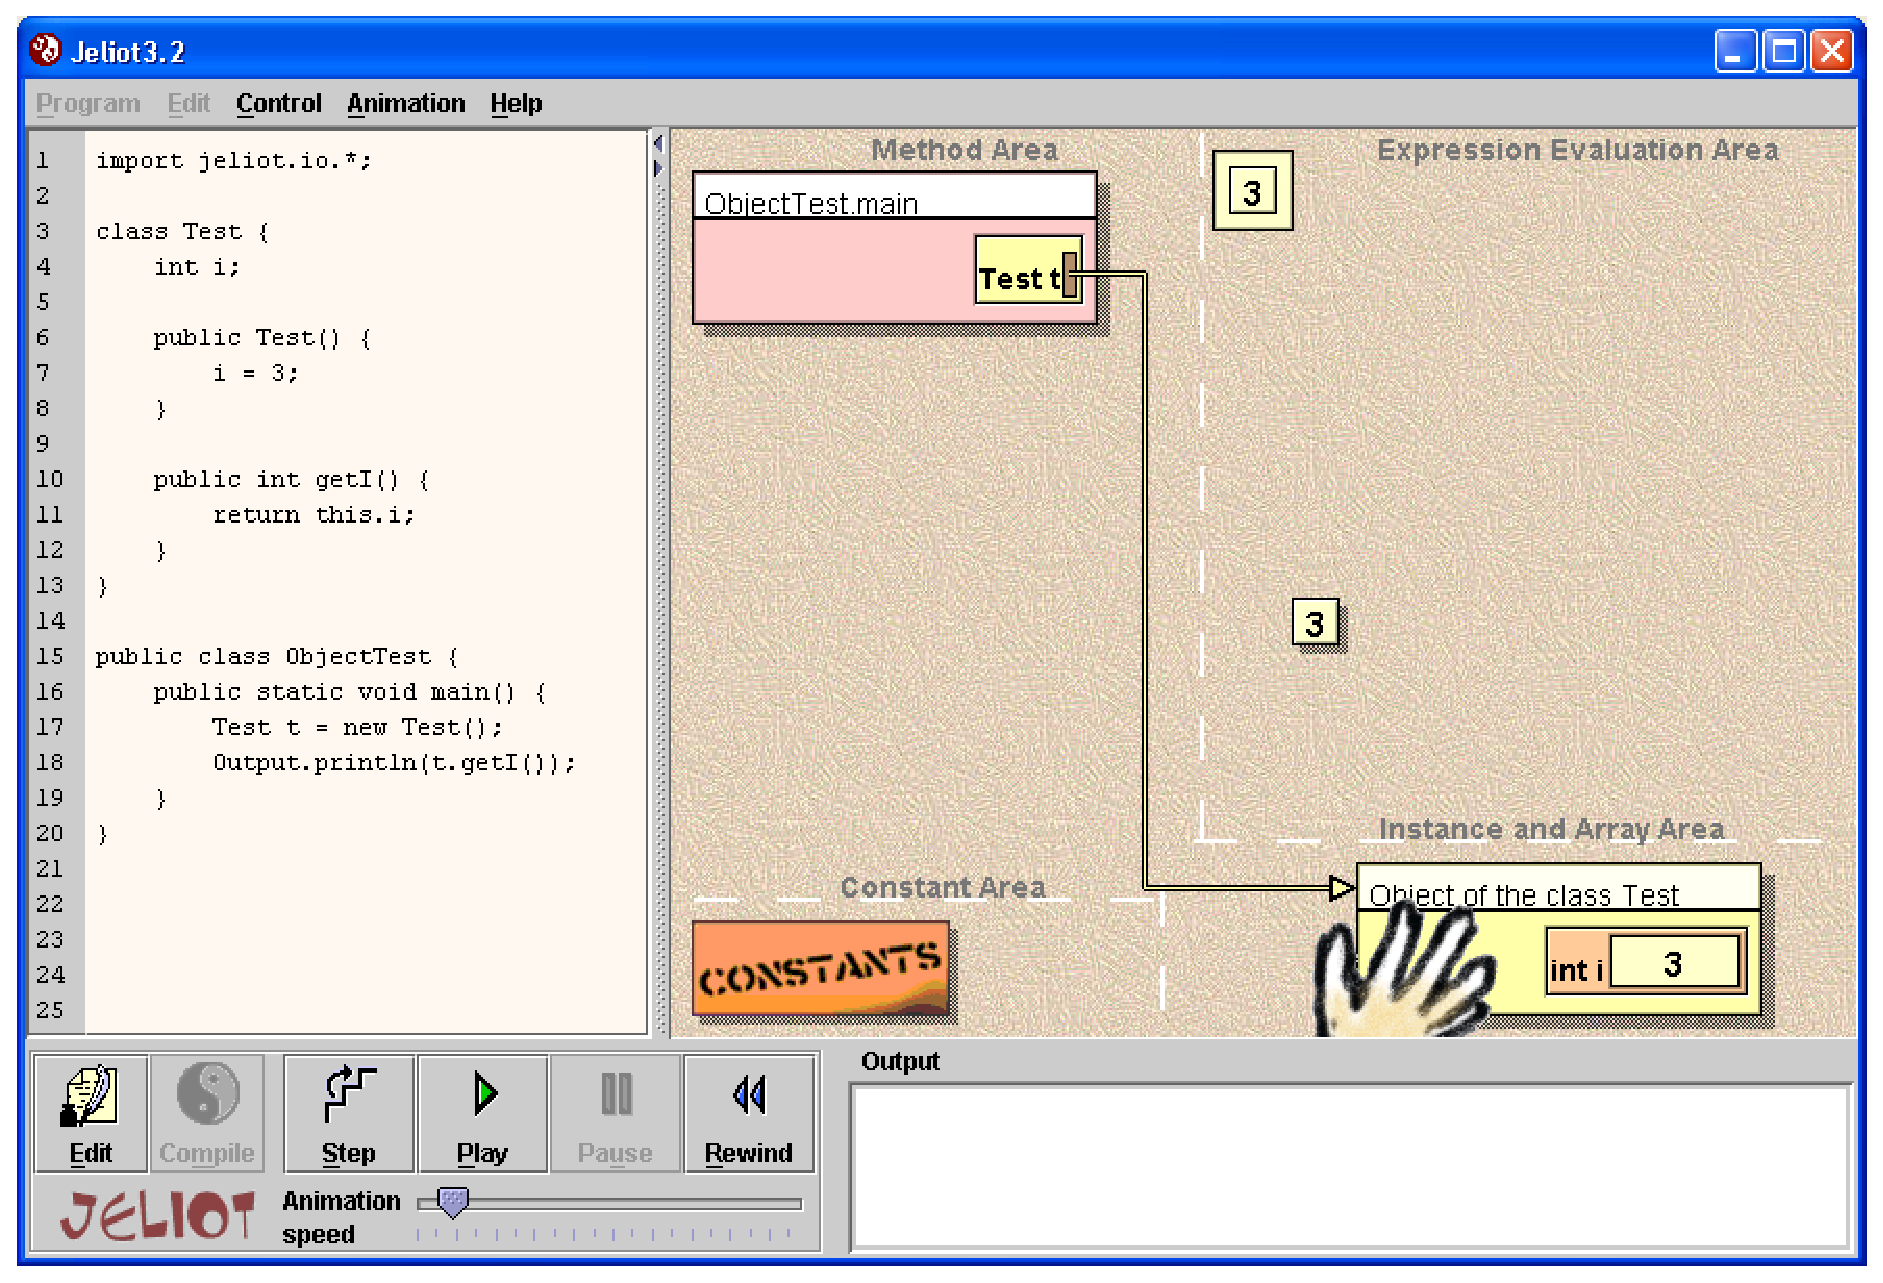
\includegraphics[width=\textwidth]{images/jeliot3.eps}
	%\vspace*{-2cm}
	%\includegraphics[width=15cm,keepaspectratio=true]{jeliot1.jpg}
	%\vspace*{-3cm}
	\caption{The \jel{} user interface and display}
	\label{fig.1}
\end{center}
\end{figure}
}

The screen is divided into a source frame on the left and an animation frame on the right. Commands may be issued from the menus or from two sets of buttons: one at the top of the screen for \hfi{}le and edit operations, and one at the bottom for animation control. All commands have mnemonics and shortcuts for quicker keyboard control. The following discussion will use the button name for each command, unless it appears only in a menu, in which case, the menu selection will be used.

The \hfi{}le commands are \bu{New}, \bu{Open} and \bu{Save}, and the edit commands are \bu{Cut}, \bu{Copy}, \bu{Paste} and \bu{Edit/Select All}. The other general commands are \bu{Help/Help}, \bu{Help/About} and \bu{File/Exit}.

\mysubsection{Editing and compiling}

When you open or create a \hfi{}le, the source code will appear in the source frame. Select \bu{Compile} to compile the \hfi{}le; if the compilation is successful, a curtain will open in the animation frame, and \jel{} will make the transition to Animation mode. If an error is found during the compilation, an error message is shown in the animation frame and the code section that (probably) contains the error is highlighted. You can return to Edit mode at any time by selecting \bu{Edit}.

\mysubsection{Animation control}

The animation is controlled by buttons at the bottom of the screen: \bu{Step}, \bu{Play}, \bu{Pause} and \bu{Rewind}. There is also a slider to control the speed of the animation. Animation may be step-by-step or continuous. Select \bu{Step} for step-by-step animation. Select \bu{Play} for continuous animation; you may stop it at any time by selecting \bu{Pause} and resume the animation by selecting \bu{Play} again. By checking the option \bu{Animation/Pause on message}, continuous animation will be stopped whenever a control statement like an \p{if}-statement is executed, and a message box describing the control action will pop up. When you select \bu{OK}, the animation continues.

\mysubsection{Animation display}

The animation is performed in the animation frame. In addition, there is an output frame at the bottom of the screen. The animation frame itself is divided into several areas:

\begin{itemize}

	\item Activation frames for each method are cascaded in the upper left hand corner. These will include the name and value of each variable.

	\item For variables of primitive or \p{String} type, the value is displayed adjacent to the name. For variables of other types, the value of the variable is a reference to an object which will be displayed at the lower right hand corner of the animation frame. A \p{null} value is displayed with an electrical ground symbol.

	\item A \emph{constant store} appears at the lower left hand corner; when an expression needs a literal, it is animated from the constant store.

	\item The upper right hand corner of the display is where expression evaluation (include method invocation) are animated. Values will be animated from the other areas and the evaluation of the expression will be carried out step-by-step. If a control statement is animated, messages will describe the outcome of the control action.

\end{itemize}

During the animation, single statements or blocks of statements will be highlighted in the source frame.

\mysection{Java issues}

There are two incompatibilities between \jel{} and standard Java.

\begin{itemize}

	\item All classes must be in a single source \hfi{}le.

	\item For I/O, import the package \p{jeliot.io.*;} which provides the methods\\
	\p{void Output.println()}, \p{int Input.readInt()}, \p{double Input.readDouble()},\\
	\p{char Input.readChar()}, \p{String Input.readString()}.

\end{itemize}

\jel{} uses DynamicJava (\url{http://koala.ilog.fr/djava/}) as a front-end and thus accepts almost all Java features that you would want to use for introductory programming, however, the implementation of the animation might not animate all features. Currently, the implementation includes:

\begin{itemize}

	\item Values of type \p{String}, all primitive types and one-dimensional arrays.

	\item Expressions including all unary and binary operations except \p{instanceof}.

	\item All the control statements (\p{if}, \p{while}, etc.).

	\item Method invocation, including recursive invocation.

	\item Constructors, allocation of objects and invocation of methods on objects.

\end{itemize}

\paragraph{Not implemented:}
\begin{itemize}

	\item Static variables.

	\item Super field accesses.

	\item Arrays with components of reference type (except \p{String})

	\item Two or more dimensional arrays.

	\item Conditional expressions (\p{exp?exp1:exp2}).

	\item Array initializers.

	\item Java 2 SDK API classes' methods cannot return object (except \p{String} type) or array types (e.g. \p{object.getClass()} that returns a \p{Class} instance).

	\item The used classes hashCode() -method has to return always a unique value.

\end{itemize}

\mysection{References}

Mordechai Ben-Ari, Niko Myller, Erkki Sutinen, and Jorma Tarhio.
Perspectives on program animation with {Jeliot}.
In {\em Software Visualization: International Seminar}, Lecture Notes
in Computer Science 2269, 31-45, Dagstuhl Castle, Germany, 2002.

Ronit {Ben-Bassat Levy}, Mordechai Ben-Ari, and Pekka~A. Uronen.
The {Jeliot} 2000 program animation system.
{\em Computers \& Education}, 40(1), 1-15, 2003.

\appendix
\newpage
\section{GNU Free Documentation License}
\addcontentsline{toc}{section}{GNU Free Documentation License}
%\label{label_fdl}

\section{GNU Free Documentation License}
\addcontentsline{toc}{section}{GNU Free Documentation License}
%\label{label_fdl}

\section{GNU Free Documentation License}
\addcontentsline{toc}{section}{GNU Free Documentation License}
%\label{label_fdl}

\input{../FDL}

\end{document}